\documentclass[titlepage]{article}
\usepackage[utf8]{inputenc}
\usepackage{hyperref}
\usepackage{float}
\restylefloat{figure}
\usepackage{color}
\definecolor{pink}{RGB}{255,102,204}
\definecolor{red}{RGB}{ 255, 51, 0}
\definecolor{orange}{RGB}{ 255, 175,30}
\definecolor{yellow}{RGB}{ 255, 255, 0}
\definecolor{green}{RGB}{ 0,176,80}
\definecolor{lgreen}{RGB}{ 146,208,80}
\definecolor{dblue}{RGB}{ 0,32,96}
\definecolor{lblue}{RGB}{ 79,129,189}

\newcommand{\pink}{\textcolor{pink}}
\newcommand{\red}{\textcolor{red}}
\newcommand{\orange}{\textcolor{orange}}
\newcommand{\yellow}{\textcolor{yellow}}
\newcommand{\green}{\textcolor{green}}
\newcommand{\lgreen}{\textcolor{lgreen}}
\newcommand{\dblue}{\textcolor{dblue}}
\newcommand{\lblue}{\textcolor{lblue}}
\usepackage{subcaption}
\usepackage{amsmath}
\usepackage{amssymb}
\usepackage{minted}
\usepackage{graphicx}
\DeclareGraphicsExtensions{.eps, .jpg, .png}
\usepackage{fancyhdr}
\pagestyle{fancy}
\lhead{Fractals and the Beauty of Nature}
\author{Chanthosh Sivanandam \\ Erik Andersen \\ Henrik Flindt }
\title{Fractals and the Beauty of Nature \\ DM550 - Fall Project 2017}
\begin{document}
\maketitle
\tableofcontents
\newpage
\section{Introduction}
While the description of a tree, triangle or a leaf is easily communicated among humans, as most humans share a common cultural understanding challenges arise when trying to convey the same idea to a computer. The task assigned in DM500 requests that a script be written which can draw different figures based upon the Fractal Description Language (FDL) in the programming language, Python, by using the Turtle module. The assignment is separated into several obligatory tasks, divided into two sections; “Fractals and the Beauty of Nature” and “Fractal Description Language''. The enterity of the source code, project files and figures can be found at \href{https://github.com/ErikAndersen81/DM550-FractalProject}{https://github.com/ErikAndersen81/DM550-FractalProject}

\section{Understanding recursion}
As an illustrative explanation of recursions, a binary-tree of a depth of four, as seen in figure \ref{fig:coltree}. The rule for the binary-tree is written as FLXRXLB, with F indicating a forward movement, B for a backward movement, and R and L as a right or left turn respectively. Each X indicates where each iteration (i.e. depth) would insert the rule. Table \ref{table:binary}  shows the four iterations from depth one to four. 
\begin{table}[H]
\centering
\caption{Rules for the binary tree}
\label{table:binary}
\begin{tabular}{lllll}
  \textbf{Depth} & \textbf{Rule}\\
  One   & F L R L B \\
  Two   & F L F L R L B R F L R L B L B\\
  Three &F L F L F L R L B R F L R L B \\
        & L R F B L F L R L B R F L R L  \\
  &B L B L B\\
  Four  & F L F L F L F L R L B R F L R\\
   & L B L B,R F L F L R L B R F L\\
   & R L B L B L B R F L F L F L R\\
   & L B R F L R L B L B R F L F L\\
   & R L B R F L R L B L B L B L B\\
  \end{tabular}
\end{table}
It should be noted that in the assignment, specifications for scaling of the length are included, but they have been removed from this example for a simple and smooth explanation. The colors in figure \ref{fig:coltree} indicate the succession of when a line is drawn. It must be stressed that the colors do not show iterations, but first passed line in a given direction, so if two or more iterations results in a line being drawn twice, only the first passing line is drawn in the figure. \newline

\begin{figure}[H]
  \caption{Binary tree with depth 4}
  \centering
  \begin{subfigure}[b]{0.4\textwidth}
    \pink{F L F L F L F L R L B} \red{R F L R L B} \pink{L B} \orange{R F L F L R L B} \yellow{R F L R L B} \orange{L B} \pink{L B} \green{R F L F L F L R L B} \lgreen{R F L R L B} \green{L B} \dblue{R F L F L R L B} \lblue{R F L R L B} \dblue{L B} \green{L B} \pink{L B}
    \caption{Color coded FDL-rule}
  \end{subfigure}
  \begin{subfigure}[b]{0.5\textwidth}
    \includegraphics[width=0.7\textwidth]{colbitree}
    \caption{Color code applied to the binary tree}
  \end{subfigure}
  \label{fig:coltree}
  \addtocounter{figure}{-1}
\end{figure}

\section{Utilizing FDL in the assignment}
The difference between one binary-tree of depth four and one binary-tree of depth 100 is only the length of the FDL and subsequent size of the tree, but the main mechanism remains unchanged.  The same mechanism would by modifying the rule, the amount of turns available, and the angle of the turns would be able to draw any figure which is shown with the Sierpinski Triangle and fern.  In this assignment additional parts have been added to the FDL mechanism that are not related to drawing lines in the Python-Turtle program, but are designed to reduce the time drawing the figure. These extra lines would in the context of the binary-tree in figure \ref{fig:coltree}  as an example enable the FDL reader to jump from the end of the red line directly to the start of the orange, the end of the yellow to jump to the green line and so forth. These jumps would either be by moving the Turtle-drawer directly or by cloning the drawing instance of Turtle to the needed point. 

\section{Trial and error}
While the final product shows a fully functional FDL readers with extra functions, minor errors in the FDL rule written would sometimes result in rather interesting figures. Figure \ref{fig:sickfern}  show a first attempt at a fern. While this is not a ideal fern, there are several signs that the underling FDL rule are on track since there are recursions in the structure and the bend is present. \par
\begin{figure}[H]
  \centering
  \includegraphics[width= .5\textwidth]{sickfern}
  \caption{Unsuccessful attempt at drawing the fern}
  \label{fig:sickfern}
\end{figure}

The first attempt took depth as a value that was transmuted in to a length that the tree and branches should cover. (In context of figure \ref{fig:coltree}  this would be the length of the pink line.) 
While this in theory would work, the math needed to ensure that the scaling would result in a tree with the correct length (len) at any given depth (x) were not found. (See figure \ref{fig:bitreesafe}  for an impression of one of the failed implementations.) The main problem were a continuous mismatch between requested depth and the printed depth of the binary-tree. \par
\begin{figure}[H]
  \centering
  \begin{minted}{python}
    x = (input('Enter depth of tree:'))
    if x.isalpha():
        exit('That is not a number!')
    x = int(round(float(x)))
  \end{minted}
  \caption{A simple safeguard}
  \label{fig:bitreesafe}
\end{figure}

The problem was overcome by adding depth as the secondary input factor in the definition of the object tree. (See figure \ref{fig:hardmath})  Length were calculated based on the request in the assignment that a tree of the depth 10 should have the length 100. The depth value x now functioned as the iteration counter while length were scaled accordingly to the branch.\par

\begin{figure}[H]
  \begin{minted}{python}
    import math
    r = 0.7
    s = 5
    len = 10 ** (math.log10(s) / x - math.log10(r)) * 5
  \end{minted}
  \caption{Hard math}
  \label{fig:hardmath}
\end{figure}

The initial attempt at drawing a fern ran in to some problems in regards to hardware limitations. While the correctness and cleanliness of the code was unquestionable, the algorithm consumed incredible amounts of ram due to several factors. One of the factors was the tremendous amounts of recursive calls. An explanation hereof is, that every time a function is called in python, the interpreter allocates memory in order to store the variables in that scope. Calling a function recursively prohibits the interpreter from freeing the allocated memory from the stack until the final function has returned its value. Furthermore, and perhaps even more malignant in terms of eating ram, was the fact that the implementation made a clone of the instance of the turtle class every time there was a new branch. While this made some clean and beautiful code, an instance of the turtle class takes up a lot of memory. Some tests showed that running the algorithm for about five to ten minutes would easily take up 30 GB of ram. On the other hand, if depth and segments where kept to a minimum, the algorithm would present a nice looking fern, yet somewhat scrawny.

\section{Binary tree}
A simple binary tree algorithm were written\footnote{The source code for this part of the project can be found in the file \href{https://github.com/ErikAndersen81/DM550-FractalProject/blob/master/Working_binary_tree.py}{binary-tree.py} or Appendix \ref{app:bintree}}, which were developed to have an option to select depth. Each time a value was calculated print statements were added for that value to ensure that troubleshooting were more easily done.  A safeguard were added to the input value x to ensure that depth would be an integer, which then would be passed down through the code. The safeguard checked for strings, and force exits if one is found. Subsequently, it rounds floats and converts them to integers. (Fig. \ref{fig:bitreesafe})
Following Turtle is imported and a few definitions of Turtle functions are written. 
Minor if statements with a print statements were added, and some modifications form the Turtle package were added for aesthetics reasons and to ensure a proper user experience. A safety question was implemented if a depth of above 12 were requested by the user. This is due to the time it takes for the tree to print, but it can be overwritten by the uses if needed.  Finally the scaffolding was removed and the script was tested for a range of depth. A binary tree of depth 10 can be seen in fig. \ref{fig:bitreeone}. \par
For this version of the binary-tree no limit for the size of the branches were implemented, since the uses might want all the branches generated, and no knowledge of the users resolution can be know in advanced.
Testing the binary tree was done to ensure a proper output. Different values for angels in the turns, and scales were tested, and depths from 1-50 were input. See figure \ref{fig:weirdtree} for four trees of depth 10, with l(25)r(60), l(45)r(80), scale 0.2 and scale 0.9. It becomes quite obvious that the predetermined values given in the assignment are optimal to render pretty binary tree as seen in figure \ref{fig:bitreeone}, when comparing this to figure \ref{fig:weirdtree}.
\begin{figure}[H]
  \centering
  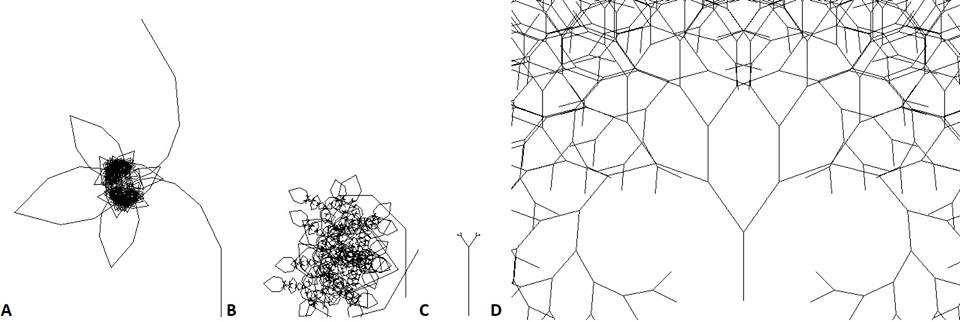
\includegraphics[width=\textwidth]{weirdtree}
  \caption{Weird trees}
  \label{fig:weirdtree}
\end{figure}
At the level of 12 the rendering time began to increase to a point where it became inconveniently to render. A second problem arose for depth of 20 plus since the crown of the tree would tend to leave the screen. A quick fix to this was implemented with some if-statements asking for a depth cap at 12. The cap is still at the user’s prerogative, so a tree with a large depth can still be generated if so required. An alternative fix would have been to change the length of the tree when the depth passed a certain value, but this will first be implemented in a later patch. "
\begin{figure}[H]
  \centering
  \includegraphics[width=0.8\textwidth]{bitreeone}
  \caption{A beautiful binary tree}
  \label{fig:bitreeone}
\end{figure}

\section{Sierpinski Triangle}
Initially, implementation of the Sierpinski triangle was build upon the idea of placing inverted triangles inside other triangles. It turned out to be a tad complicated, but it yielded some rather interesting results, which can be seen in \ref{fig:unsuccessful1} and \ref{fig:unsuccessful2}
\begin{figure}[H]
  \centering
  \caption{Not Sierpinski's triangles}
  \begin{subfigure}[b]{0.4\textwidth}
    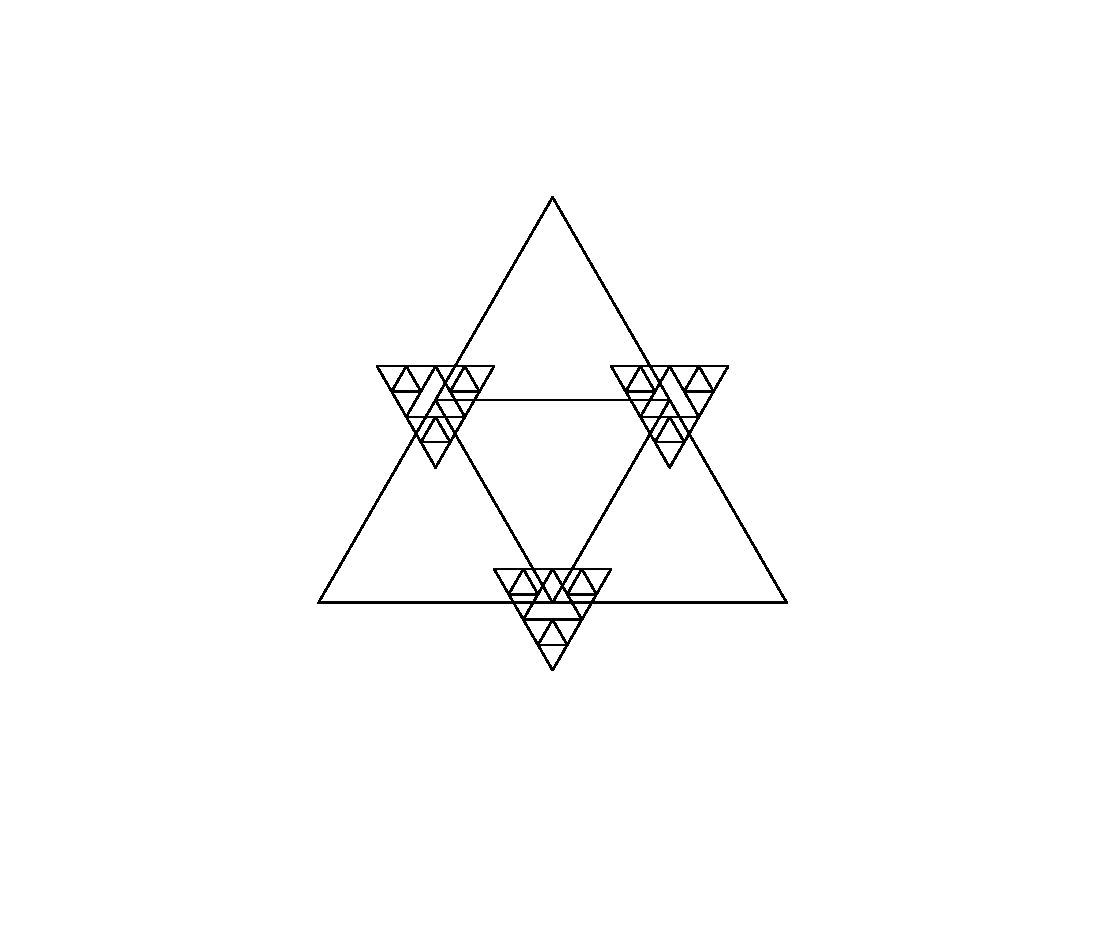
\includegraphics[width=\textwidth]{wrongtriangle}
    \caption{An unsuccessful attempt}
    \label{fig:unsuccessful1}
  \end{subfigure}
  \begin{subfigure}[b]{0.5\textwidth}
    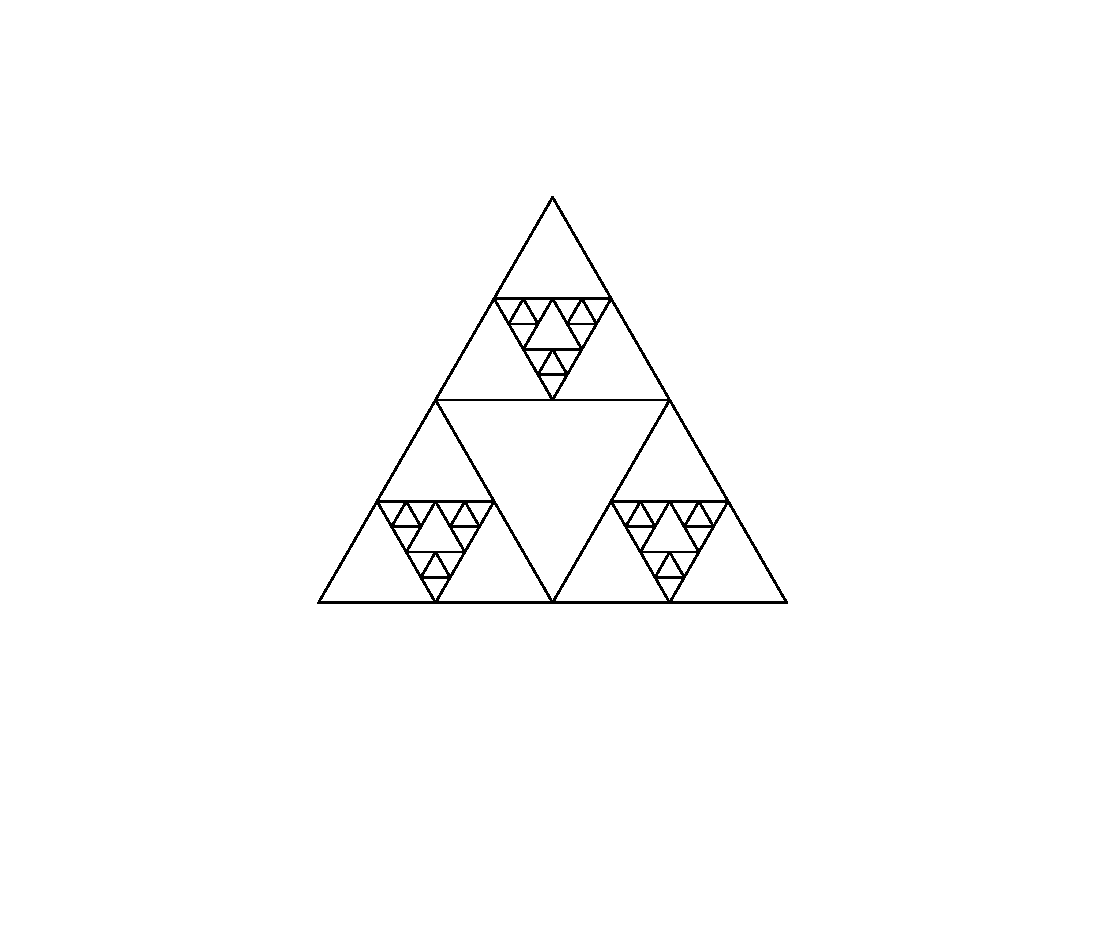
\includegraphics[width=\textwidth]{wrongtriangle2}
    \caption{Another unsuccessful attempt}
    \label{fig:unsuccessful2}
  \end{subfigure}
  \addtocounter{figure}{-1}
\end{figure}
After meddling around for some time, a decision was made to try the approach suggested in the project description. A successful algorithm that gave the expected result was then rapidly developed.
\begin{figure}[H]
  
  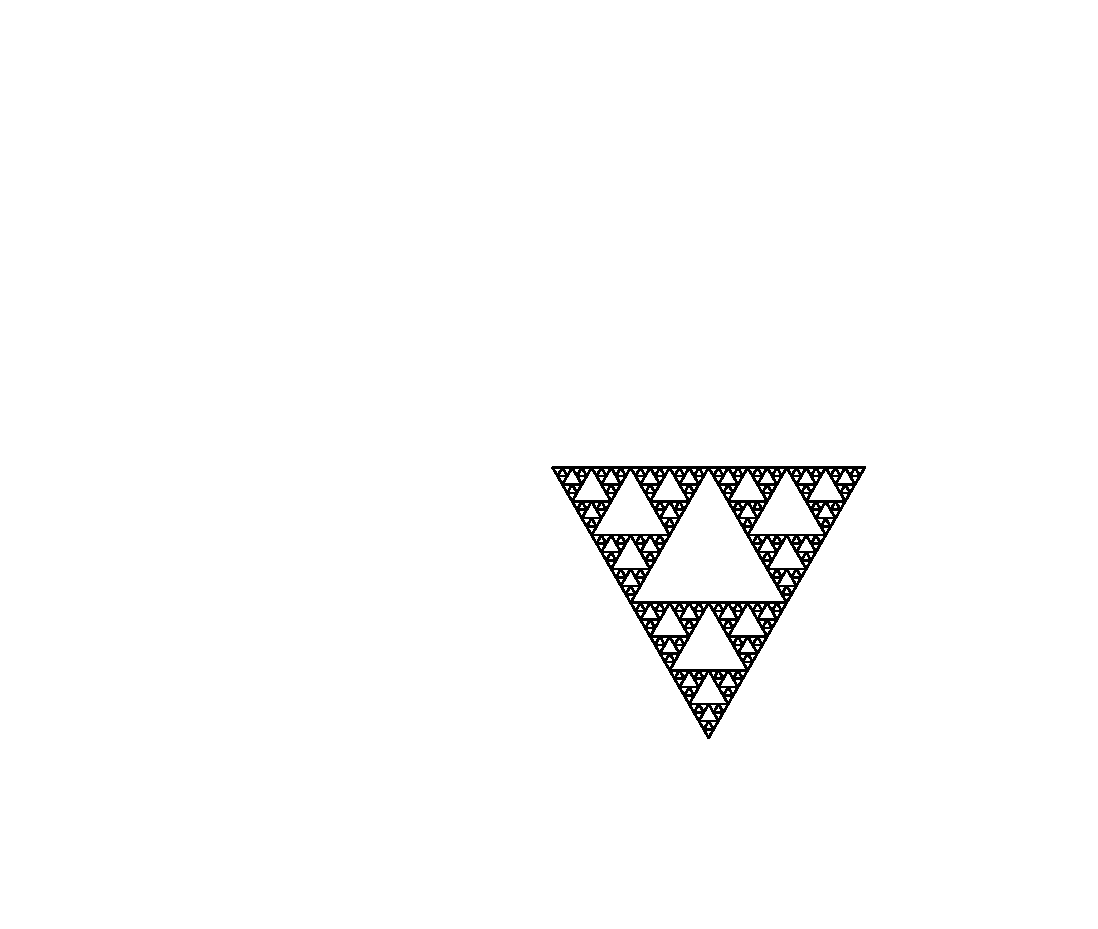
\includegraphics[width=0.6\textwidth]{triangle}
  \caption{Sierpinski triangle with 5 subdivisions.}
\end{figure}
Revisiting the initial code, the faultiness of its algorithm became apparent and hence could be corrected. The effectiveness of this new code compared to the approach recommended in the project description is due to the lack of redundant drawing. \par We used an iterative development process, meaning we started out by making a small piece of the code work in one iteration. Through testing, trial and error the goal of the iterative step was reached and we then carried on with the next step, where more code was implemented and tested. After several steps, we realized that our approach was overly complicated, so we started again from scratch. This time we did not care for optimization of the algorithm, and we solely focused on correctness.\footnote{The source code for this part of the project can be found in the file \href{https://github.com/ErikAndersen81/DM550-FractalProject/blob/master/sierpinsky-triangle.py}{sierpinsky-triangle.py} or appendix \ref{app:sierpinski}}

\section{Fern}
The idea was to create a program that illustrate a fern graphically. Eventually, Afterwards with some time we were able to find the ground principle illustrating the fern. The program was made and were supposed to draw the first part of the stalk, then turn left and draw the leaves and sub-leaves. When the first side of the leaf the program heads back to the position. It draws the right side of the leaf and sub-leaves and every time it was drawing a leaf or sub-leaf the angle gets 0,3 smaller, then it returns to the position and goes forward and repeats itself, until the steps eventually goes down to zero.

Eventually, it was easier to divide the fern into smaller pieces and named them. Eventually, the function were made with some necessary parameters for creating the fern. The parameters in the function are the turtle module, the width (thickness of each line), the segments, the curve (angle every time we draw the next leaf) and steps is the length of the fern frond \ref{fig:frond}. There were a lot of trials making the program recursive, because the posistion was not returning to the stalk, so the position were made with a turtle method.\par
\begin{figure}[H]
  \centering
  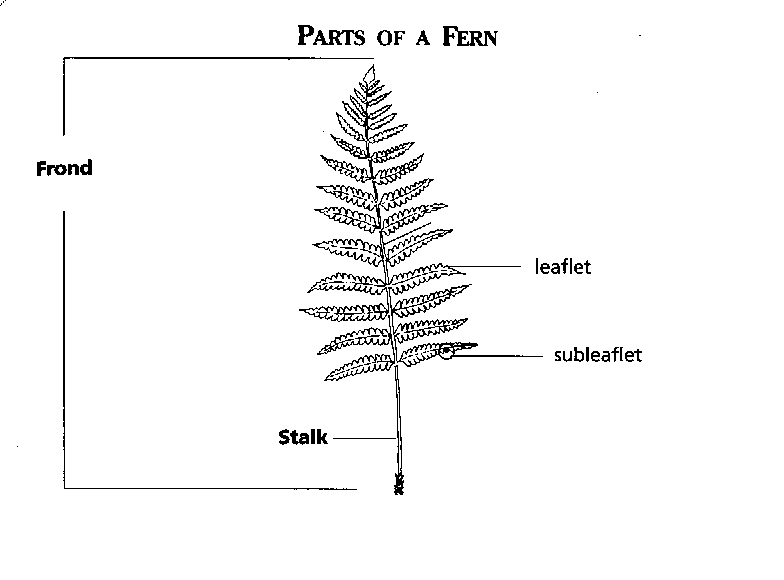
\includegraphics[width=\textwidth]{Fern}
  \caption{Fern}
  \label{fig:frond}
\end{figure}
Generally, the function were created for the stem on the fern with several important parameters (length, width, segments curve, steps). To illustrate the segments the for-loop was a necessary method. The way for-loops work is for statement iterates over the segments of a sequence in order, executing the block each time. The pen size is the width of each line, in other words it is the thickness of the leaves and sub-leaves. And every time it goes to the next step the width downsizes with 0,3. the curve is the angle each time we go to the next sub-leaves and the stalk is also turn a bit to the left. At this point we had some difficulty because it did not have any position and return when the sub-leaves were drawn. There were used two methods called position and heading. The first method is a way too return the current position (x,y) which is very useful when it were able to return back to the stalk and go forward. The other method is the heading which returns the turtle direction.
\par
At the beginning there were a lot of trials because there were some difficulty making it recursive. after several approach there was a idea that divides the fern into smaller pieces and make the program for each piece and put them together. But at the end it made it too hard to assemble the pieces together. Finally, At the end there were made a function with all the parameters that worked with recursion. While with some realisation that the run time was way too long to execute, Because of the long runtime we began to create another fern with a different method called clone and it worked, however run time was fast but because the clone method uses a lot of memory the execute time takes way too much time. \footnote{The source code for this part of the project can be found in the file \href{https://github.com/ErikAndersen81/DM550-FractalProject/blob/master/fern.py}{fern.py} or appendix \ref{app:fern}}


\begin{minted}{python}  
def recursive_stem(t, length, width, segments, curve, steps):
    if steps == 0:
        return
    if length < 0.5:
        return
    for i in range(segments):
        t.pensize(width)
        t.lt(curve)
        t.fd(length)
        pos=t.pos()
        head=t.heading()
        t.rt(90)
        recursive_stem(t, length*0.3, width*0.3, segments, curve, steps-1)
\end{minted}

\section{FDL-Parser}
Since the fdl-file is to be read by an instance of the turtle module's Turtle class, it was decided to make a subclass of it called SmartTurtle. This class should be able to read a fdl-file, and execute he commands, giving a reasonable result. Through analysis of several fdl-files, a decision as to which attributes the SmartTurtle class should implement, could be made. Thus, an instance of the SmartTurtle should have a \textit{start} attribute containing a command, a \textit{length}, a \textit{depth}, a dictionary of \textit{rules}, and one of commands (\textit{cmd}) which could be called with appropriate arguments. The rules should be unfolded according to the depth of the SmartTurtle, which seemed to indicate that an \textit{unfolded} attribute would be convenient. This attribute would initially be an empty string, but when the user of the SmartTurtle class would want to execute the commands in the fdl-file loaded, a function to unfold the rules list and store them as a string in the unfolded attribute, will be required. This functionality is implemented in SmartTurtle's \textit{step} function. The parser basically just reads through each line of the file, recognizing keywords, like \textit{start}, \textit{rule} and the like. The keywords are then used as look-ups in the dictionary yielding a string containing arguments, list of rules, or a float or int, depending on the type of keyword. 

\section{Conclusion}
Trial and error seemed to yield the expected results, and in the process a fully functional fdl-parser was developed. There could be several optimizations in regards to a more user friendly interface and faster rendering of the fractals. Most of these optimizations should probably not be implemented using the turtle module, but perhaps with the help of the matplotlib module. Furthermore, in regards to increasing the speed of execution, some of the code could presumably be written in Cython or plain c/c++ and then utilized as an extension to python.

\appendix
\section{Appendix}
\subsection{Binary tree}
\label{app:bintree}
\inputminted{python}{binary-tree.py}
\begin{figure}[H]
  \centering
  \includegraphics{bintreeleaves}
  \caption{The output of binary-tree.py}
\end{figure}
\subsection{Sierpinski's Triangle}
\label{app:sierpinski}
\inputminted{python}{sierpinsky-triangle.py}
\subsection{Fern}
\label{app:fern}
\inputminted{python}{fern.py}
\begin{figure}[H]
  \centering
  \includegraphics[width=\textwidth]{myfern}
  \caption{The output of fern.py}
\end{figure}
\subsection{FDL-Parser}
\inputminted{python}{fdlParser.py}
\end{document}
